\documentclass[12pt]{article}
\usepackage{parskip}
\usepackage{amsmath}
\usepackage{pdfpages}
\usepackage[margin=.6in]{geometry}

\begin{document}	
\includepdf[pages=2]{slides}
Instead of saying I have a problem to solve and I will come up with a solution, we have to let a computer solve the problem and learn to do it so well that it beats us.

\includepdf[pages=5]{slides}
\includepdf[pages=6]{slides}
Say we have a large system, we can simplify it to two simple states. This is trying to predict what the next state of the system will be. 

\includepdf[pages=7-33]{slides}


\includepdf[pages=35]{slides}
We want to be able to see what the next prime number is. Prediction is great.
































\end{document}